\documentclass[
	classe=$2^{de}$,
]{exercice}

\usepackage{tcolorbox}
\usepackage{tikz-repère}
\usetikzlibrary{calc}

\newcommand{\Point}[3]{#1(\correctionOr{{\color{red}#2}}{\phantom{3333}};\correctionOr{{\color{red}#3}}{\phantom{3333}})}

\title{Activité : chronophotographie}

\begin{document}

\maketitle

\begin{tcolorbox}
	Une \textbf{chronophotographie} est un procédé qui consiste à prendre en photo un mouvement à intervalle réguliers.

	On peut ensuite étudier la superposition de ces photographies pour déterminer la trajectoire et la vitesse d'un objet donné.
\end{tcolorbox}

\section*{Chronophotographie}

\begin{enumerate}
	\item Sur le document distribué :

	      \begin{itemize}
		      \item Choisir une partie du corps qui soit visible à chaque instant.
		      \item Suivre la position de cette partie, en la marquant de croix sur la photo.
		      \item Numéroter les points obtenus dans l'ordre.
	      \end{itemize}
	\item Donner la liste des coordonnées obtenues dans le repère $(O ; \vec{i}, \vec{j})$ :
	      \begin{multicols}{4}
		      \begin{itemize}
			      \setlength{\itemsep}{0.5em}
			      \item $\Point{P₀}{}{}$
			      \item $\Point{P₁}{}{}$
			      \item $\Point{P₂}{}{}$
			      \item $\Point{P₃}{}{}$
			      \item $\Point{P₄}{}{}$
			      \item $\Point{P₅}{}{}$
			      \item $\Point{P₆}{}{}$
			      \item $\Point{P₇}{}{}$
		      \end{itemize}
	      \end{multicols}
	\item On va maintenant calculer la vitesse avec des vecteurs : si il y a $t$ temps entre chaque photo, pour calculer la vitesse à la $n$-ième photo, on doit calculer $\dfrac{1}{t} × \vec{PₙP_{n+1}}$.

	      Placer ainsi sur le document la vitesse correspondant à chaque point (sauf le dernier).
\end{enumerate}

\section*{Chute libre}

Sur le schéma ci-dessous, on a représenté la trajectoire d'un objet en chute libre : il y a $2$ secondes d'intervalle entre chaque positions.

\begin{center}
	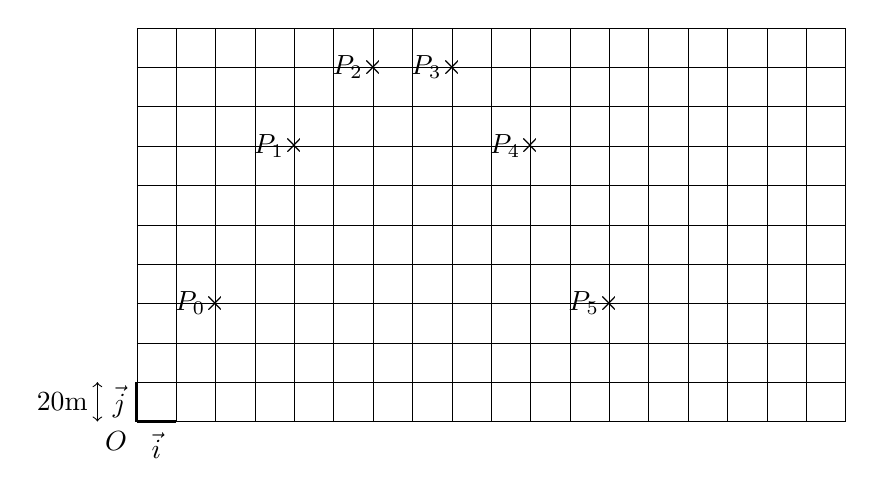
\begin{tikzpicture}[scale=0.5]
		\coordinate (BasGauche) at (0,0);
		\draw[ultra thin] (BasGauche) grid ++(18,10);
		\draw[<->] (BasGauche) ++(-1,0) -- node[left] {$20$m} ++(0,1);
		\node[below left] at (BasGauche) {$O$};
		\draw[very thick,\myArrow] (BasGauche) -- node[below] {$\vec{i}$} ++(1,0);
		\draw[very thick,\myArrow] (BasGauche) -- node[left] {$\vec{j}$} ++(0,1);

		\coordinate (P) at (40,60);
		\coordinate (V) at (20,40);
		\coordinate (A) at (0,-10);
		\foreach \i in {0,...,5} {
				\node[thick] at ($0.05*(P)$) {×};
				\node[thick,left] at ($0.05*(P)$) {$P_{\i}$};
				\ifdefined\makeCorrection
					\draw[red,\myArrow] ($0.05*(P)$) -- node[above] {$\vec{v_{\i}}$} ++($0.05*(V)$);
				\fi
				\coordinate (P) at ($(P) + 2*(V)$);
				\coordinate (V) at ($(V) + 2*(A)$);
			}
	\end{tikzpicture}
\end{center}

\begin{enumerate}
	\item Quelle est la direction du mouvement de l'objet ici ?
	\item Lire les coordonnées de chaque point dans le repère $(O ; \vec{i}, \vec{j})$ :

	      \begin{center}
		      \begin{multicols}{6}
			      $\Point{P₀}{15}{10}$
			      \columnbreak
			      $\Point{P₁}{35}{25}$
			      \columnbreak
			      $\Point{P₂}{55}{30}$
			      \columnbreak
			      $\Point{P₃}{75}{15}$
			      \columnbreak
			      $\Point{P₄}{95}{10}$
			      \columnbreak
			      $\Point{P₅}{95}{10}$
		      \end{multicols}
	      \end{center}
	\item Pour calculer la vitesse $\vec{vₜ}$ au temps $t$, on utilise la formule $\vec{vₜ} = \dfrac{1}{t}\vec{P_{t+1}Pₜ}$

	      Placer alors $\vec{v₀}$, $\vec{v₁}$, $\vec{v₂}$ et $\vec{v₃}$ sur le repère.
	\item Calculer les vecteurs variations de vitesse $Δ\vec{v₀} = \vec{v₁} - \vec{v₀}$ et $Δ\vec{v₂} = \vec{v₃} - \vec{v₂}$. Que remarque-t'on ?
\end{enumerate}

\end{document}